\chapter{Identifying candidate novel ncRNAs from \textit{Psa} transcriptomes}
\label{chap:psa_ncRNA}

\section{Preface}

Successful pathogenic bacteria must alter gene expression in response to changing and hostile environments. Non-coding RNAs (ncRNAs) contribute to adaptability by forming complex regulatory networks, and contribute to the survival and virulence of pathogens. 

As of yet no studies have been undertaken to extensively characterise ncRNA genes in \textit{Pseudomonas syringae} pv. \textit{actinidiae}. We have generated transcriptomes of a New Zealand strain of \textit{Psa} in multiple growth conditions \textit{in vitro}, and used this data, as well as previously generated \textit{in planta} transcriptomes, to identify candidate ncRNAs, with the aim of identifying those involved in infection and virulence. With this data we have identified transcripts that are highly expressed in specific growth conditions, and which have predicted secondary structure motifs characteristic to known functional ncRNAs. We have also characterised the expression pattern of annotated ncRNAs in \textit{Psa}, and identified that an uncharacterised RNA motif, twoAYGGAY, is highly prevalent in the \textit{Psa} genome.

\subsection{Contributions}
I performed all data analysis. RNA-seq generation is described in Chapter 4.
\newpage


\section{Introduction}

Bacterial genomes contain a multitude of functional non-coding RNA (ncRNA) genes. These include small ncRNAs (sRNAs), short transcripts which often have some secondary structure, and predominantly function as regulators of gene or protein expression by base-pairing with mRNA transcripts. Many sRNAs are only expressed under specific growth conditions, and can be found as key regulators of pathogenic responses in bacteria, including those that infect plants.

\textit{Pseudomonas syringae} pv. \textit{actinidiae} (\textit{Psa}) is a plant pathogen that causes kiwifruit canker disease, which has had a significant impact on the New Zealand kiwifruit industry. Mutations in the RNA chaperone Hfq, which is required to stabilise many sRNA-mRNA interactions, is linked to reduced virulence in the pandemic strain of \textit{Psa}, suggesting sRNAs play a role in virulence in this organism \citep{Zhao2019}.

Transcriptomic screens have identified sRNAs in other Pseudomonads \citep{GomezLozano_2012,GomezLozano_2015}, notably in \textit{P. syringae} pv. \textit{tomato} DC3000, where a non-coding transcript was found to regulate the biosynthesis of the phytotoxin coronatine \citep{Filiatrault_2010x,Geng2014-jh}. In other plant pathogens sRNAs have been found to be important regulators of pathogenicity. In \textit{Erwinia carotovora}, RsmB regulates enzymes that degrade plant cell walls, and the horizontally-acquired sRNA-Xcc1 discovered in \textit{Xanthomonas campestris} is a regulator of virulence factors \citep{Liu_1998x,Chen_Tang_2011x}. 

Novel ncRNAs can be identified by measuring expression in intergenic regions \citep{Rath_Pitman_Cho_Bai_2017x,Lindgreen_Umu_2014x}, with the incorporation of conservation and structural information providing useful signals to identify candidates that are likely to be functional \citep{Stav_Atilho_Mirihana_2019x}. Recent approaches for the comprehensive identification of ncRNAs have used exhaustive multi-condition transcriptomics, which has been effective in identifying ncRNAs relevant to pathogenicity in \textit{E. coli} \citep{Rau2015-xxgt} and \textit{Salmonella} \citep{Kroger_Hokamp_2013x}.

More targeted experiments have also been performed in \textit{Pseudomonas aeruginosa} to identify strain and species-specific sRNAs \citep{Ferrara_2012x}, as well as temperature-dependent sRNA expression \citep{Wurtzel_Lory_2012x}. However, the phylogenetic distribution of many sRNAs are limited, and many sRNAs with specialised functions are genus, strain or niche-specific, due to both rapid evolution and sequence gain and loss of ncRNA genes through horizontal gene transfer \citep{Jose2019-xxxu}. This trend can also be seen in \textit{P. aeruginosa} sRNAs, few of which have known homologues in \textit{P. syringae} \citep{GomezLozano_2015}.

In this study, transcriptomes from \textit{Psa} generated in multiple growth conditions were used to predict candidate ncRNAs, aiming to identify ncRNAs relevant to pathogenicity. Sequences from manual ncRNA annotations were tested for differential gene expression between \textit{Psa} transcriptomes grown \textit{in vitro} in rich, starved and minimal media, and were also compared to transcriptomes of \textit{Psa} grown \textit{in planta} generated by \cite{McAtee_2018x}.

\section{Methods}

\subsection{ncRNA annotation}

\textit{In vitro} and \textit{in planta} RNA-seq reads (see Chapter 4 for experimental details) were processed using \texttt{trimmomatic} v0.36 \citep{Bolger_Usadel_2014x}, and mapped to the \textit{Pseudomonas syringae} pv. \textit{actinidiae} ICMP 18884 chromosome and plasmid sequences (NCBI accession CP011972.2 and CP011973.1) \citep{Templeton2015-mx} using Bowtie2 v2.3.4 \citep{Langmead2012x}. \texttt{Samtools} v1.8 \citep{Li_Handsaker_Wysoker_Fennellx} was used to generate plot files representing the number of reads mapped to each nucleotide (Figure \ref{fig:peak_example}). 

Candidate ncRNAs were manually annotated using the Artemis genome viewer \citep{Carver_Harris_Berriman_Parkhill_McQuillan_2012x}. 
Plot files were used to visualise read depth across the genome for each experiment. Expression peaks in intergenic regions, or opposite protein coding genes, that were over 50 nt in length and with a read depth of at least 50 in \textit{in vitro} samples and over 10 in \textit{in planta} samples that were similarly expressed between replicates were considered candidate ncRNAs. 

While small protein-coding elements are a feature of some ncRNAs, this was considered a confounding factor for the conservation analysis. Expression peaks for likely protein-coding candidates and UTRs are included in supplemental materials. To ensure that predicted ncRNAs located in intergenic regions did not overlap with un-annotated genes, pseudogenes or small ORFs, the reference genome was re-annotated with \texttt{Prokka} \citep{Seemann_2014x}, \texttt{cmscan} with Rfam models \citep{Nawrocki_Burge_Bateman_Daub_Eberhardt_Eddy_Floden_Gardner_Jones_Tate_2015x} and \texttt{RNIE} \citep{Gardner_Barquist_Bateman_Nawrocki_Weinberg_2011x}. Protein domain annotations were generated from a 6-frame translation the genome, which was annotated using \texttt{HMMER} \citep{Eddy2011-chi} and Pfam HMMs \citep{Punta_Coggill_2012x}. For ncRNA annotations found only in the unstranded \textit{in planta} RNA-seq data, terminators and protein coding genes were used to infer strand where applicable. Known ncRNAs were annotated using Rfam domains; as many of these annotations were partial, expression peaks were used to estimate transcription start sites.

\begin{figure}[H]
    \centering
    \includegraphics[scale=1]{psa/psa_ncRNA/peak_example.png}
    \caption[Example showing the visualisation of RNA-seq counts and candidate ncRNA annotation in the Artemis genome browser]{Example showing the visualisation of RNA-seq counts and annotations of candidate ncRNAs in the Artemis genome browser. Panels A and B show traces representing the number of RNA-seq reads mapped to the \textit{Psa} genome. \textbf{(A)} \textit{In vitro} traces each represent a single replicate and are coloured based on experiment conditions. The two windows show reads mapping to the forward and reverse strands. \textbf{(B)} Traces representing \textit{in planta} samples. Due to the low read depth of the \textit{in planta} data, each trace represents the sum across a set of replicates, with an additional trace added representing the sum across all \textit{in planta} samples (shown in red). \textbf{(C)} Gene and genome feature annotations (shown in frame). Two protein-coding genes (blue) and an annotated tRNA are expressed. Dotted lines show an expression peak in an intergenic region, which would be classified as a candidate ncRNA.}
    \label{fig:peak_example}
\end{figure}

\subsection{Quality control}

\subsection{Sequence uniqueness}

BLAST \citep{Altschul1990-knr} was used to check whether candidate ncRNA sequences were homologous to each other, or contained sequences that were non-unique in the genome. A reciprocal \texttt{blastn} search was used between all candidate ncRNAs to look for multi-copy or common motifs. This showed that 18 sequences were homologous to at least one other candidate ncRNA. These clustered into five groups, which could be classified by shared sequence motifs and/or similarity of function of nearby genes. \texttt{Cytoscape} \citep{Shannon2003-uv} was used to visualise groups of homologous sequences (Figure \ref{fig:cytoscape}). 
The largest cluster of candidate ncRNAs were found upstream of group II introns. Several of these candidates also had homology to genomic regions containing an annotated Rfam motif, twoAYGGAY, which was also often upstream of group II introns.

A \texttt{blastn} search of these candidates against the genome identified that the ncRNA sequences in the UTRs of oxidoreductases and ABC transporters, and twoAYGGAY-like sequences were highly multi-copy throughout the genome. These were not included in the conservation analysis.  


\subsection{Conservation analysis}

A homology search was performed to assess whether any candidate ncRNA sequences were conserved within \textit{Pseudomonas} genomes, using an iterative \texttt{nhmmer}-based \citep{Wheeler2013-qlw} approach described previously (Methods, Chapter 3). A database of whole \textit{Pseudomonas} genomes was created, consisting of 489 complete genome and plasmid sequences from NCBI. Candidate ncRNA sequences were used to generate single-sequence profile HMMs using \texttt{hmmbuild}, which were used in an \texttt{nhmmer} homology search of 63 \textit{Pseudomonas syringae} genomes in the database. These sequences were then aligned using the ncRNA alignment tool \texttt{mafft-qinsi} \citep{Katoh2013x}, built into new HMMs and searched over all \textit{Pseudomonas} genomes. Multiple sequence alignments for each candidate were made from the final homology search results.

\begin{figure}[H]
    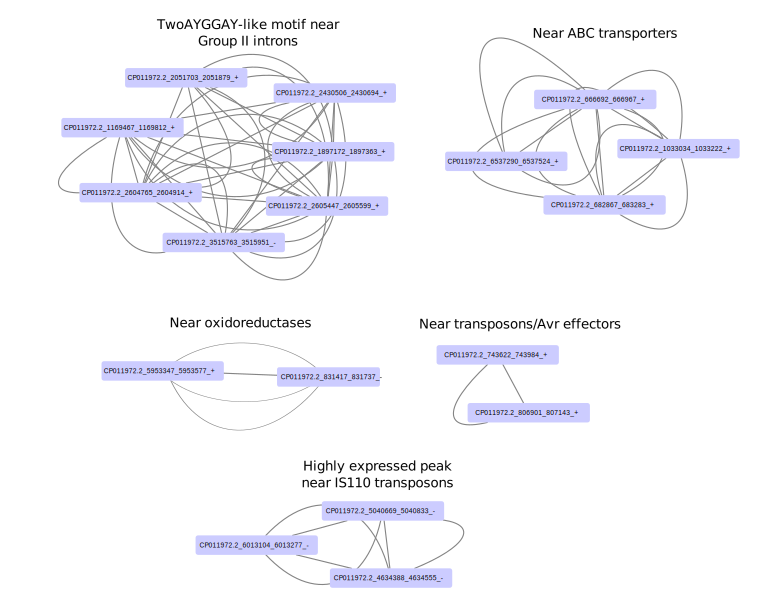
\includegraphics[scale=0.8]{psa/psa_ncRNA/all_v_all.png}
    \caption[Network diagram showing annotated ncRNAs with high sequence similarity to each other]{Network diagram showing annotated ncRNAs with high sequence similarity to each other. Networks are generated from an all vs all \texttt{blastn} search of candidate ncRNAs. Nodes are individual ncRNAs, and edges represent instances of a significant \texttt{blastn} hit to another ncRNA. Clusters are labelled based on their context in the \textit{Psa} genome and visualised in \texttt{Cytoscape} \citep{Shannon2003-uv}.}
    \label{fig:cytoscape}
\end{figure}

\subsection{Alignment analysis and structure prediction}

Several tools were used to identify alignments that were most likely to be non-coding RNAs (Figure \ref{fig:psa_flowchart}). \texttt{RNAcode} was used to test if candidate ncRNAs had protein coding potential \citep{Washietl2011x}; 20 candidates with a p value < 0.01 were removed. \texttt{Alifoldz} was used to identify alignments that had significant signals of stable secondary structure \citep{Washietl2004-pk}. Conserved candidate ncRNAs with negative z-scores were selected. For alignments with few sequences or little sequence variation, \texttt{alifoldz} z-score, \texttt{RNAalifold} secondary structures and alignments were manually inspected to select candidates.

\texttt{RNAalifold} \citep{Bernhart_Hofacker_Will_Gruber_Stadler_2008x} was used to predict a consensus secondary structure for each alignment. Six conserved candidates that did not have a thermodynamically favourable secondary structure (minimum free energy of > -20) were removed. \texttt{R-scape} \citep{Rivas_Clements_Eddy_2017x} was used to identify covarying base-pairs within predicted secondary structures. Six structures containing covarying base-pairs with an E-value < 0.01 were selected as final candidates. \texttt{R-scape} tests could not be applied to alignments with limited numbers of sequences. Thermodynamic stability and covariance scores, conservation and expression were used to select and rank the final ncRNA candidates. For candidates with limited phylogenetic distribution, MFE, overall expression and differential expression were used to select the final candidates. Secondary structures were visualised using R2R \citep{Weinberg2011-nxxx}.
\subsection{Differential gene expression and expression in other data-sets}
Candidate intergenic ncRNAs as well as Rfam annotations were tested for differential expression using \texttt{Kallisto} (settings$:$ \texttt{ -b 100 $--$rf-stranded}) \citep{Bray2016-xxoi} and DESeq2 \citep{Love2014-dccv} using the same analysis pipeline as Chapter 4 (see Appendix x for details). 

Publicly available data on the Sequence Read Archive (https://www.ncbi.nlm.nih.gov/sra) was used to find paired-end, stranded \textit{Pseudomonas} RNA-seq data-sets. Metadata from the NCBI FTP server was used to generate a table consisting of SRA accession, SRA experiment number, sequencing design (paired or single-end reads), read length, sequencing instrument, NCBI biosample, NCBI taxonomy ID, organism genome accession and species name. This table was then used to select seven \textit{P. syringae} pv. \textit{tabaci} ATCC 11528 (\textit{Pta}) transcriptomes (Table \ref{tab:tabaci_transcriptomes}, Table \ref{tab:tabaci_transcriptomes_2}), generated \textit{in vitro} in M9 media, which were used to test if candidate ncRNAs were expressed in other organisms.

Profile HMMs of candidate ncRNAs, which were generated from alignments generated during the conservation analysis, were used to annotate the \textit{Pta} genome ATCC 11528 (NCBI Accession ACHU02.1). Sequencing reads were mapped to the genome and visualised using the same pipeline as the \textit{Psa} transcriptomes (Appendix x). Homology search results were then used find sequences homologous to \textit{Psa} candidate ncRNAs in the \textit{Pta} genome that also showed similar levels of expression. 
\begin{figure}[H]
\begin{minipage}{0.6\textwidth}
    \includegraphics[scale=1]{psa/psa_ncRNA/flowchart3.png}
\end{minipage}
\begin{minipage}{0.39\textwidth}
    \caption[Flow-chart showing showing quality control steps used to select final candidate ncRNAs]{Flow-chart showing showing quality control steps used to select final candidate ncRNAs. Briefly, manual annotations that were single copy were selected for conservation analysis. Multiple sequence alignments from this homology search were then tested for signals that would identify the candidates as functional ncRNAs. \texttt{RNAcode} was used to test if sequences were likely to be protein coding \citep{Washietl2011x}, and \texttt{alifoldz} z-scores and \texttt{RNAalifold} minimum free energy (MFE) was used to identify candidates with thermodynamically stable predicted secondary structure \citep{Bernhart_Hofacker_Will_Gruber_Stadler_2008x,Washietl2004-pk}. Additional tests were placed on conserved sequences (>12 sequences) using \texttt{R-scape} \citep{Rivas_Clements_Eddy_2017x}. Manual curation removed a further 8 candidates based on poor expression and conservation, maintenance of synteny, biased sequence composition and conservation of secondary structure.}
    \label{fig:psa_flowchart}
\end{minipage}
\end{figure}




\begin{table}[H]
    \footnotesize
    \centering
    \begin{tabular}{p{3cm}cccp{6cm}}\toprule
SRA Accession &  Platform & Read length & Paired? & Experiment conditions\\\midrule
SRR3747530, SRR3747531&HiSeq 2500& 125 &Yes & M9 media, 5mM mannitol\\
SRR3747532, SRR3747533& HiSeq 2500& 125 &Yes & M9 media, 5mM mannitol, C\textsubscript{6}-HSL\\
SRR3747538, SRR3747539& HiSeq 2500& 125 &Yes & M9 media, 5mM mannitol, 3OC\textsubscript{6}-HSL\\

\bottomrule
    \end{tabular}
    \caption[\textit{Pta} transcriptomes used to validate candidate ncRNA expression (SRP078028)]{Publicly available transcriptomes from \textit{Pta} ATCC 11528 (SRP078028), used to validate expression of conserved candidate ncRNAs identified in \textit{Psa}. Data generated by \cite{Cheng2018-eo}. }
    \label{tab:tabaci_transcriptomes}
\end{table}

\begin{table}[H]
    \footnotesize
    \centering
    \begin{tabular}{p{2.5cm}cccp{6cm}}\toprule
SRA Accession &  Platform & Read length & Paired? & Experiment conditions\\\midrule
SRR3757176, SRR3757178, SRR3757179 & HiSeq 2000 & 101 & Yes & KB media, exponential/stationary phase \\
SRR3757150, SRR3757153, SRR3757154 & HiSeq 2000 & 101 & Yes & KB media, exponential phase \\
SRR3757099, SRR3757100, SRR3757106 & HiSeq 2000 & 101 & Yes & KB media, lag phase \\
\bottomrule
    \end{tabular}
    \caption[\textit{Pta} transcriptomes used to validate candidate ncRNA expression (SRP078136)]{Publicly available transcriptomes from \textit{Pta} ATCC 11528 (SRP078136), used to validate expression of conserved candidate ncRNAs identified in \textit{Psa}. Data generated by \cite{Cheng2017-ja}. }
    \label{tab:tabaci_transcriptomes_2}
\end{table}

%data was shitty !
%\begin{table}[H]
%    \footnotesize
%    \centering
%    \begin{tabular}{p{2.5cm}cccp{6cm}}\toprule
%SRA Accession &  Platform & Read length & Paired? & Experiment conditions\\\midrule
%ERR973046 & HiSeq 2000 & 102 & Yes & Swarming plates \\
%ERR973047 & HiSeq 2000 & 102 & Yes & MMR minimal media \\
%\bottomrule
%    \end{tabular}
%    \caption{Publically available transcriptomes from \textit{Pseudomonas syringae} pv. %\textit{tomato} DC3000, used to validate expression of conserved candidate ncRNAs identified in \textit{Psa}. Data generated by \cite{Nogales2015-pj}. }
%    \label{tab:tomato_transcriptomes}
%\end{table}
\section{Results and Discussion}

Manual annotation identified 94 intergenic and 137 antisense expression peaks as candidate ncRNAs. Rfam-guided annotations of known ncRNAs identified gene boundaries for 54 small ncRNAs, as well as a class of 46 ncRNA sequences with twoAYGGAY-like motifs. Rfam domains were also used to identify 56 group II intron-derived sequences, although it is unclear what proportion of these remain intact or functional.

\subsection{TwoAYGGAY-like motifs in \textit{Psa} and \textit{Pseudomonas}}

Seven intergenic peaks annotated as novel ncRNAs were identified near group II introns. These sequences had high sequence similarity to each other, Rfam-annotated twoAYGGAY motifs, as well as intergenic regions which were not expressed in this experiment. Overall 43 motifs were annotated$:$ Rfam identified 12 motifs, which increased to 36 after removing the --cut-ga thresholding during annotation (E-value threshold = 0.01). Others were identified by an nhmmer homology search, using a HMM generated from an alignment of manually annotated twoAYGGAY-like sequences. An alignment of all twoAYGGAY and twoAYGGAY-like sequences had a highly stable Y-shaped predicted secondary structure, which is similar to the Rfam twoAYGGAY motif (Figure \ref{fig:twoAYGGAY_genomic}). Motif-containing sequences within the \textit{Psa} genome are generally highly similar, and have covarying sites maintaining secondary structure.   

\begin{figure}[H]
    \centering
    \includegraphics[scale=1.25]{psa/psa_ncRNA/multi-twoayggay.png}
    \caption[Consensus predicted secondary structure of twoAYGGAY-like candidate ncRNAs, and example of tandem twoAYGGAY-motifs in \textit{Psa}]{\textbf{(A)} Consensus predicted secondary structure of candidate ncRNAs homologous to annotated twoAYGGAY ncRNAs in the \textit{Psa} genome. Candidates were aligned using \texttt{mafft-qinsi} and consensus secondary structure predicted with \texttt{RNAalifold}. \textbf{(B)} Example showing tandem repeats of the twoAYGGAY-like motif in \textit{Psa}. Bottom panel shows genome annotations. \textbf{Pink:} Motifs, \textbf{Green:} Annotated group II intron, \textbf{Blue:}  Protein annotations. Top panel shows RNA-seq counts for \textit{in vitro} and \textit{in planta} data-sets. A set of 4 tandem repeats can be seen on the forward strand at the 5$\textprime$ end of the group II intron, and a single motif at the 3$\textprime$ end. Motif annotations closest to the ends of the group II intron are palindromic, generating annotations on each strand. Annotations were visualised in the Artemis genome browser.}
    \label{fig:twoAYGGAY_genomic}
\end{figure}

The \textit{Psa} twoAYGGAY-like sequences do not have the 5$\textprime$-AYGGAY-3$\textprime$ sequence in the terminal loops, but do contain 5$\textprime$-GGA-3$\textprime$ motifs, which is consistent with the binding site of Csr/Rsm-binding RNAs \citep{Gardner2015-co}. TwoAYGGAY-like motifs were commonly found throughout the \textit{Psa} genome in intergenic regions, often near group II introns. Several intergenic regions have tandem repeats of this motif, and 26 sequences were sufficiently palindromic that they were annotated in the same location on both strands.  

Conservation analysis of the most highly expressed sequence which contained the twoAYGGAY-like motif (CP011972.2, 1897172-1897363) found that this sequence is highly conserved throughout \textit{Pseudomonas} genomes. Consensus secondary structure of sequences from the homology search is generally similar to the Rfam twoAYGGAY predicted secondary structure, but has a shorter and more variable P1 stem, a shorter P2 stem, small unpaired bulges, and a 5$\textprime$-AUGGAU-3$\textprime$
motif in the terminal loops (Figure \ref{fig:twoAYGGAY_conserved}). 

\begin{figure}[H]
    \centering
    \includegraphics[scale=0.4]{psa/psa_ncRNA/TwoAYYGAY_example.png}
    \caption[Comparison of predicted consensus secondary structure of twoAYGGAY-like motifs and the Rfam twoAYGGAY motif]{\textbf{Left:} Predicted consensus secondary structure of twoAYGGAY-like motifs in \textit{Pseudomonas} genomes. An alignment was generated by an iterative nhmmer homology search from a single twoAYGGAY-like sequence over Pseudomonas genomes. \textbf{Right:} Rfam consensus secondary structure for the twoAYGGAY motif.}
    \label{fig:twoAYGGAY_conserved}
\end{figure}

The function of these motifs are unclear, although the conservation of secondary structure and Csr/Rsm binding motif suggests they may function in the sequestration of Csr/Rsm RNA-binding proteins \citep{Gardner2015-co}. These motifs were also associated with group II introns (p = 0.008, Fisher's exact test, Table \ref{tab:fisher}). 

Group II introns have been observed to insert near palindromic motifs in \textit{P. putida} KT2440 \citep{Yeo2001-gg}, and similar palindromic elements, including ncRNAs, are often insertion sites for other mobile genetic elements \citep{Darmon2014-dxj,Dai2002-fm}. It may be that this sequence is associated with the re-homing of introns, however, the mechanisms of re-homing and transposition of bacterial group II introns are diverse and not well understood \citep{Dai2002-fm}, and their recognition sites are highly variable \citep{Lambowitz2011-oq}.
\begin{table}[H]
    \centering
    \begin{tabular}{c|cc}

         & TwoAYGGAY & Group II intron \\
        \midrule
         Adjacent & 28 & 21\\
         Independent & 15 & 35\\

         Total & 43 & 56 \\

    \end{tabular}
    \caption[Contingency table showing the association of twoAYGGAY-motifs with group II introns]{Contingency table showing the association of twoAYGGAY-motifs with group II introns. These are classified into 'adjacent', where a twoAYGGAY annotation is in an intergenic region up- or down-stream of a group II intron, and 'independent' where flanking gene annotations are not part of group II introns. For regions containing multiple clustered twoAYGGAY repeats, all repeats in the same intergenic region are classed as adjacent or independent.}
    \label{tab:fisher}
\end{table}


%Previous studies of Group II intron transposition in \textit{P. putida} found that intron transposition often ocurred next to hairpin loops, which were later identified as repetitive extragenic palindromic (REP) elements \citep{Aranda-Olmedo2002-zoc}. Several sequence regions in the \textit{Psa} TwoAYGGAY-like motifs contain the GCGGG..CCCGC sequence common to the \textit{P. putida} REP motifs \citep{Yeo2001-gg}.
%The previous observation of insertion event near the Csr-binding ncRNA \textit{rsmZ} in \textit{P. putida} KT2440 \citep{Joardar2005-uj} suggests that insertion near
\subsection{Intergenic candidate ncRNAs}

Overall 71 annotated intergenic candidates were selected for conservation analysis. Quality control of the final alignments of homologous sequences removed 21 candidates that had predicted protein coding potential, 26 conserved ncRNAs with a positive \texttt{alifoldz} z-score, and 7 candidates that did not have thermodynamically stable predicted secondary structures. In total, 36 candidate ncRNAs passed alignment quality control. The conservation of these sequences and preservation of synteny was used to attempt to classify gene origins. During manual curation 4 candidates were classed as pseudogenes due to homology with proteins and tRNAs in other genomes and were removed, and another 4 were removed due to inconsistent conservation of secondary structure. 

Most candidate ncRNAs were poorly conserved; 7 were specific to \textit{Psa}, and another 7 associated with mobile genetic elements were primarily found in {Psa} with a small number of annotations to sequences near the same MGEs present in other species. Many poorly conserved candidates were located in regions created by recent re-arrangements in the \textit{P. syringae} or \textit{Psa} lineages. Several of these had highly stable predicted secondary structures, however these were part of highly repetitive and palindromic intergenic regions, which may be remnants of previous transposition events. While rearrangements can cause the creation of novel transcripts, it is difficult to identify if these are functional ncRNAs or transcriptional noise \citep{Jose2019-xxxu}. Other poorly conserved candidate ncRNAs were associated with mobile genetic elements such as transposons and integrases, reiterating results from the conservation analysis of \textit{Salmonella} sRNAs in Chapter 3. 

\begin{table}[H]
    \footnotesize
    \centering
    \begin{tabular}{ccccc}\toprule
Name &  Sequence & Start & End & Strand\\\midrule
Psa_sRNA_003 & CP011973.1 & 21610 & 21774 & -\\
Psa_sRNA_004* & CP011973.1 & 61084 & 61315 & -\\
Psa_sRNA_005* & CP011973.1 & 61080 & 61307 & +\\
Psa_sRNA_006 & CP011972.2 & 170583 & 170708 & -\\
Psa_sRNA_007* & CP011972.2 & 806901 & 807143 & +\\
Psa_sRNA_009 & CP011972.2 & 6082989 & 6083300 & -\\
Psa_sRNA_010* & CP011972.2 & 6513384 & 6513635 & -\\
Psa_sRNA_011 & CP011972.2 & 743622 & 743984 & +\\
Psa_sRNA_012 & CP011972.2 & 3765999 & 3766298 & -\\
Psa_sRNA_013* & CP011972.2 & 1752191 & 1752476 & +\\
Psa_sRNA_014 & CP011972.2 & 3260267 & 3260449 & +\\
Psa_sRNA_015 & CP011972.2 & 739233 & 739548 & -\\
Psa_sRNA_016 & CP011972.2 & 760028 & 760267 & +\\
Psa_sRNA_017 & CP011972.2 & 2294607 & 2294819 & -\\
Psa_sRNA_018 & CP011972.2 & 5148068 & 5148376 & +\\
Psa_sRNA_019 & CP011972.2 & 768152 & 768370 & +\\
Psa_sRNA_020* & CP011972.2 & 2035568 & 2035765 & +\\
Psa_sRNA_021* & CP011972.2 & 119433 & 119810 & +\\
Psa_sRNA_022 & CP011972.2 & 119724 & 119882 & -\\
Psa_sRNA_023 & CP011972.2 & 1494687 & 1495064 & -\\
Psa_sRNA_024* & CP011972.2 & 4634388 & 4634555 & -\\
Psa_sRNA_025* & CP011972.2 & 5040669 & 5040833 & -\\
Psa_sRNA_026$\dagger$ & CP011972.2 & 1300899 & 1301216 & -\\
Psa_sRNA_027* & CP011972.2 & 745275 & 745542 & -\\
Psa_sRNA_028*$\dagger$ & CP011972.2 & 322030 & 322306 & +\\
Psa_sRNA_029* & CP011972.2 & 5438181 & 5438417 & -\\
Psa_sRNA_031$\dagger$ & CP011972.2 & 5459360 & 5459656 & +\\
Psa_sRNA_032$\dagger$ & CP011972.2 & 5469984 & 5470208 & +\\
\bottomrule
    \end{tabular}
    \caption[Genome locations of final candidate ncRNAs]{Final candidate ncRNAs and genome locations. \textbf{*} indicates that this transcript is either adjacent to or part of a mobile genetic element. \textbf{$\dagger$} denotes candidates that were found to be expressed in \textit{Pta}.}
    \label{tab:final_canditates}
\end{table}
Final candidates (Table \ref{tab:final_canditates}) were ranked by conservation, overall expression, expression in other data-sets, the presence of condition-specific expression and differential expression (Figure \ref{fig:candidate_heatmap}). Three were expressed only \textit{in vitro}, four were only expressed \textit{in planta}, two in minimal media only and one in rich log samples only. One candidate Psa\_sRNA\_012, was significantly differentially expressed across \textit{in vitro} data-sets (P\textsubscript{adj} < 0.01). 

\begin{figure}[H]
    \centering
    \includegraphics[scale=0.95]{psa/psa_ncRNA/final_candidates_heatmap2.png}
    \caption[Sequence conservation and expression of candidate ncRNAs]{Heatmap showing the annotation range and sequence conservation of intergenic candidate ncRNAs annotated in \textit{Psa} across \textit{Pseudomonas} genomes. Sequence conservation is shown as a colour gradient from blue (100\%) to red (40\%), representing genus average percent sequence identity based on alignment to the sequence from \textit{P. syringae} pv. \textit{actinidiae} ICMP 18884. Gene conservation is shown as a change in opacity, represented by the percentage of genomes with an annotation within that genus. Genes are ordered based on overall conservation. Additional panels show expression data for these genes. \textbf{Top:} Basemean from \textit{in vitro} RNA-seq calculated by DEseq2. \textbf{Middle:} Peak max of mapped reads from \textit{in planta} plot files, which is the maximum combined read depth from all \textit{in planta} plot files across the annotated region. Both panels are capped at 1000. \textbf{*} Denotes candidate ncRNAs located in the \textit{Psa} ICMP 1884 plasmid, \textbf{$\dagger$} denotes candidates that are differentially expressed \textit{in vitro}}
    \label{fig:candidate_heatmap}
\end{figure}
\newpage

Candidates that were associated with mobile genetic elements were in general more highly expressed in starvation conditions. High expression of the protein components of these MGEs was also observed in the same conditions (Chapter 4), indicating these transcripts may be under the same regulatory mechanisms. 

Psa\_sRNA\_022 was highly expressed under starvation conditions and \textit{in planta}, and found next to a hypothetical protein. Additional annotation of this hypothetical protein found homology to the Abi$/$CAAX family of transmembrane metalloproteases \citep{Kjos2010-yq}, which are involved in self-immunity to bacteriocins, and have been found as part of a cassette of resistance genes carried by toxin-antitoxin systems in \textit{Staphylococcus} \citep{Bukowski2017-gd}.  A small expression peak adjacent to this candidate was also detected. Annotations in strains outside \textit{Psa} found that Psa\_sRNA\_022 was located at the 5$\textprime$ end of a CAAX protease. This locus appears to have been disrupted in \textit{P. syringae} due to an integration or transposition event (Figure \ref{fig:srna_022_operon}). This transcript had a conserved secondary structure with a GNRA tetraloop, which are structural motifs that can form and stabilise tertiary structure \citep{Fiore2013-mf}. 

 \hfill
\begin{figure}[H]
    \centering
    \includegraphics[scale=1.5]{psa/psa_ncRNA/sRNA_022.png}
        \caption[Comparison of the Psa\_sRNA\_022 locus in \textit{Psa} and \textit{P. rhizophaerae}]{Comparison of the region containing Psa_sRNA_022 sequence in \textit{Psa} and a homologous sequence in \textit{P. rhizosphaerae} strain DSM 16299. \textbf{Top:} \textit{P. rhizosphaerae} locus containing Psa\_sRNA\_022 (blue), next to a CAAX protease. \textbf{Bottom:} \textit{Psa} locus containing Psa\_sRNA\_022, which is located between two hypothetical proteins (yellow) with homology to CAAX protease. }
    \label{fig:srna_022_operon}
\end{figure}
\begin{figure}[H]
\begin{subfigure}{0.49\textwidth}
\includegraphics[scale=0.7]{psa/psa_ncRNA/psa_srna_022_exp.png} 
\end{subfigure}
\begin{minipage}{0.49\textwidth}
\includegraphics[scale=0.8]{psa/psa_ncRNA/sRNA_022_structure.png}
    \caption[Expression and predicted consensus secondary structure of Psa\_sRNA\_022]{\textbf{Left:} Expression peak for Psa\_sRNA\_022. This region is highly expressed in starvation conditions \textit{in vitro} and is expressed \textit{in planta}. \textbf{Right:} Predicted consensus secondary structure for Psa\_sRNA\_022.}
    \label{fig:srna_022}
    \end{minipage}
\end{figure}

Psa\_sRNA\_032, located downstream of a plasmid partitioning protein ParA and conjugation machinery, was highly constitutively expressed in \textit{Psa} and all \textit{Pta} samples (Figure \ref{fig:srna_032}). This candidate was found primarily in \textit{P. syringae} pv. \textit{actinidiae}, and was homologous to intergenic regions near mobile genetic elements in 3 genomes outside of \textit{P. syringae}. This transcript appears to have a stable secondary structure, containing conserved stem-loops (Figure \ref{fig:srna_032}). The context and high constitutive expression of this transcript suggests it may be a regulator or part of a Par plasmid-maintaining toxin-antitoxin system \citep{Muthuramalingam2019-uy}.

\begin{figure}[H]
\centering
    \includegraphics[scale=1.05]{psa/psa_ncRNA/tabaci_and_psa.png}
    \begin{minipage}{0.6\textwidth}
\includegraphics[scale=0.9]{psa/psa_ncRNA/sRNA_032.png}
    \end{minipage}
    \begin{minipage}{0.39\textwidth}
    \caption[Expression of a Psa\_sRNA\_032 in \textit{Psa} and \textit{Pta}]{\textbf{Top:} Expression of Psa\_sRNA\_032 in \textit{Psa} and expression of a homologous sequence in \textit{Pta}. Psa\_sRNA\_032, which is in a locus that is conserved in both genomes is highly constitutively expressed in \textit{Psa} grown \textit{in vitro} and \textit{in planta} (\textbf{left}), and also expressed in two data-sets of \textit{Pta} grown \textit{in vitro} (\textbf{right}). Peaks are smaller in \textit{Pta} due to variations in read depth between data-sets. \textbf{Bottom:} Predicted consensus secondary structure for Psa\_sRNA\_032.}
    \label{fig:srna_032}
    \end{minipage}
\end{figure}

Psa\_sRNA\_006, which is weakly expressed \textit{in vitro} and \textit{in planta}, was found in multiple Pseudomonas species and had a highly conserved secondary structure (Figure \ref{fig:srna_006}), containing two GNRA tetraloops and a highly significant covarying base-pair (E-value = 0.0003). This candidate was located near siderophore export channels in \textit{Psa}, and was homologous to a horizontally-acquired region in \textit{P. aeruginosa} near the type IV pili regulator \textit{hrpB}. 

\begin{figure}[H]
\begin{subfigure}{0.4\textwidth}
\includegraphics[scale=0.67]{psa/psa_ncRNA/psa_srna_006_exp.png} 
\end{subfigure}
\begin{minipage}{0.59\textwidth}
\includegraphics[scale=0.9]{psa/psa_ncRNA/srna_006.png}
    \caption[Expression and predicted consensus secondary structure of Psa\_sRNA\_006]{\textbf{Left:} Expression peak for Psa\_sRNA\_006. This region is weakly expressed \textit{in planta}. \textbf{Right:} Predicted consensus secondary structure for Psa\_sRNA\_006, showing highly conserved stem-loops, containing covarying base-pairs.}
    \label{fig:srna_006}
    \end{minipage}
\end{figure}

Psa\_sRNA\_026 was conserved throughout \textit{P. syringae} and found in several closely related Pseudomonas species. This candidate was only expressed in minimal media \textit{in vitro} and was highly expressed \textit{in planta}, and is located in a conserved intergenic region located upstream of alginate biosynthesis genes, and next to a metal-sensing peroxide stress protein YaaA \citep{Liu2011-rz}. The predicted consensus secondary structure for Psa\_sRNA\_026 was highly structured, however several peripheral stem-loops were not highly conserved (Figure \ref{fig:srna_026}).

\begin{figure}[H]
    \centering
\includegraphics[width=0.9\linewidth]{psa/psa_ncRNA/psa_srna_026_exp.png} 
\end{figure}
\begin{figure}[H]
    \centering
\includegraphics[width=0.75\linewidth]{psa/psa_ncRNA/sRNA_026.png}
    \caption[Expression and predicted consensus secondary structure for Psa\_sRNA\_026]{\textbf{Top}: Expression of Psa\_sRNA\_026 in \textit{Psa}, where it is expressed in minimal media \textit{in vitro}, and \textit{in planta}. Expression in \textit{Pta} is also shown. \textbf{Bottom}: Predicted consensus secondary structure for Psa\_sRNA\_026.}
    \label{fig:srna_026}
\end{figure}

\subsection{Psa\_sRNA\_031 is a \textit{Pseudomonas syringae} \textit{pesA} homologue}
Homology search results showed that Psa\_sRNA\_031 was conserved across \textit{Pseudomonas}, including several strains of \textit{P. aeruginosa}, a well-studied human pathogen and model organism. The \textit{Pseudomonas} transcriptome browser by \cite{Wurtzel_Lory_2012x} was used to identify that an intergenic region in \textit{P. aeruginosa} str. PA14 that is homologous to Psa\_sRNA\_031 was highly expressed (Figure \ref{fig:p_browser}) and has been identified as a small RNA. This transcript, named PesA (previously known as SPA0021), is located in the PAPI-4 pathogenicity island found in many pathogenic strains of \textit{P. aeruginosa}, and may act in \textit{trans} to attenuate the expression of the bacteriocin, pyocin S3 \citep{Ferrara2017-su}. PesA also improves survival and stress tolerance in response to UV, however the mechanism for this is unclear \citep{Ferrara2017-su}. 

\begin{figure}[H]
    \centering
    \includegraphics[scale=0.8]{psa/psa_ncRNA/pseudomonas_browser.png}
    \caption[Expression of a Psa\_sRNA\_031 homologue in \textit{P. aeruginosa}] {Data from the Pseudomonas RNA-seq browser \citep{Wurtzel_Lory_2012x}), showing expression of a region homologous to Psa\_sRNA\_031 the in \textit{P. aeruginosa} str. PA14 (PA14\_sr\_128). This region overlaps with the annotated sRNA \textit{pesA}, located at 5288100-5288500 in this genome \citep{Pita2018-bi}. The Pseudomonas RNA-seq browser is located at $http://www.weizmann.ac.il/molgen/Sorek/pseudomonas\_browser/$ }
    \label{fig:p_browser}
\end{figure}

The expression of \textit{pesA} appears to be regulated differently in \textit{P. syringae} strains than in \textit{P. aeruginosa}. PesA expression is induced at body temperature in \textit{P. aeruginosa}, however it is constitutively expressed across the \textit{Psa} and \textit{Pta} RNA-seq data-sets used in this study. 

Conservation analysis and structural prediction showed that both the nucleotide sequence and secondary structure of PesA are conserved across \textit{Pseudomonas} genomes (Figure \ref{fig:pesa_structure}), with an average sequence identity of 89\% and lowest sequence identity of 71\% between \textit{Psa} and \textit{P. protogens} sequences. A sequence region of \textit{pesA} that has been predicted to be the interaction site with the pyocin S3 mRNA ribosomal binding site in \textit{P. aeruginosa} (UUCUCCCUGUGUCUCCCUGUUCUUUUGCUUGUC) was conserved across all sequences, with some variability in the 3$\textprime$ end (Figures \ref{fig:pesa_structure} and \ref{fig:pesa_binding_site}). 

\begin{figure}[H]
    \centering
    \includegraphics[scale=1.8]{psa/psa_ncRNA/Pesa_binding_site.png}
    \caption[Predicted consensus structure of PesA]{Predicted consensus structure of PesA with the experimentally confirmed mRNA binding region from \textit{P. aeruginosa} highlighted (yellow).}
    \label{fig:pesa_structure}
\end{figure}

In \textit{P. aeruginosa} and \textit{P. protegens}, \textit{pesA} is found next to genes encoding Type IV pili, however in  \textit{P. syringae} and other \textit{Pseudomonas} plant pathogens (\textit{P. avenellae}, \textit{P. amygdali} and \textit{P. cerasicola}) \textit{pesA} is located next to a DNA topoisomerase III in PacICE1, a integrative conjugative element circulating among \textit{Pseudomonas} in the Pacific \citep{Colombi2017-zf,Colombi2017-yxxf}. 
%Pacific-specific ICE 5410644	5511601 in CP011972.2
\begin{figure}[H]
\includegraphics[scale=0.9]{psa/psa_ncRNA/PesA_binding_site_conservation_2.png}
    \caption[Sequence logo showing nucleotide conservation across the PesA binding site]{Sequence logo showing nucleotide conservation across the PesA binding site. Image generated by WebLogo (https$:$//weblogo.berkeley.edu/logo.cgi)}
    \label{fig:pesa_binding_site}
\end{figure}


\begin{wrapfigure}{l}{0.5\textwidth}
\centering
    \includegraphics[scale=0.72]{psa/psa_ncRNA/pesa_iyo_017970.png}
    \caption[CopraRNA predicted interaction between Psa\_sRNA\_031 and IYO\_017970]{Visualisation showing the top predicted interaction between Psa\_sRNA\_031 (\textit{pesA}) and \textit{Psa} mRNAs generated by CopraRNA \citep{Wright2014-vh,Wright2013-cc}. Interacting regions of the predicted conserved binding region of PesA and a region upstream of the start codon of IYO_017970  are shown. Figure generated with RNAplot \citep{Lorenz2011-wt}. }
    \label{fig:copraRNA}
\end{wrapfigure}To investigate if \textit{pesA} functions in pathogenicity in \textit{P. syringae}, CopraRNA \citep{Wright2014-vh,Wright2013-cc} was used to predict conserved interactions between PesA and mRNA sequences in 4 \textit{P. syringae} strains, \textit{P. syringae} pv. \textit{actinidiae} ICMP 18884 (NCBI accession: NZ\_CP011972), \textit{P. syringae} pv. \textit{syringae} B728a (NCBI accession: NC\_007005), 
\textit{P. syringae} pv. \textit{tomato} str. B13-200 (NCBI accession: NZ\_CP019871) and \textit{P. syringae} pv. \textit{atrofaciens} str. LMG5095 (NCBI accession: NZ\_CP028490). CopraRNA high scoring interactions (Table \ref{tab:COPRARNA}) include stress genes that are required for survival \textit{in planta}, indicating that PesA may have an analogous role in promoting survival in plant hosts. The top-scoring interaction with an arylesterase, an enzyme which is involved in the degradation of carboxylic and phenolic esters \citep{Wang2010-fs}, which are present in many plant-derived compounds such as salicyclic acid and lignin. Phenolic compounds have been shown to induce the expression of \textit{hrp} virulence and T3SS genes in \textit{P. syringae} pv. \textit{tomato} \citep{Lee2015-ub}. The ArnA interaction with PesA was predicted to interact with the previously identified PesA binding site (Figure \ref{fig:copraRNA}). Other targes include UDP-glucoronic acid oxidase ArnA, which is involved in LPS synthesis \citep{Breazeale2002-cd}, and PhnA, which is involved in the uptake of alkylphosphonates, which are phosphate-containing compounds that include some fungicides and herbicides \citep{Chen1990-ql}. Other targets include the ribosomal protein RpsO, which binds to the 16S RNA and has been found to interact with sRNAs in \textit{E. coli} \citep{Fontaine2016-go}, and UspA, which is a conserved components of many stress responses \citep{Kvint2003-kg}.

%Describe how copraRNA works

%\begin{figure}[H]
%    \centering
%    \includegraphics[scale=0.7]{psa/psa_ncRNA/PesA_sRNA_regions_with_histogram.pn}
%    \caption{Histogram of predicted interaction regions of the \textit{P. syringae pesA} homologues with mRNAs. The top predicted interaction is highlighted in red, which overlaps with the previously predicted pesA binding site.}
%    \label{fig:my_label}
%\end{figure}
%\begin{figure}[H]
%    \centering
%    \includegraphics[scale=0.7]{psa/psa_ncRNA/PesA_mRNA_regions_with_histogram.png}
%    \caption{Histogram of predicted interaction regions of mRNAs interacting with \textit{pesA}. For this analysis, only the region 200 nt upstream and 100 nt downstream of each mRNA was analysed. The top predicted interaction is highlighted in blue.}
%    \label{fig:my_label}
%\end{figure}

%, sRNApredict2 \citep{Cao2009-hf} was used to identify potential targets for PesA in \textit{P. syringae} pv. B728a. Three of the top-ranked results were predicted to interact with the binding site previously identified in \textit{P. aeruginosa} (Figure \ref{fig:pesa_targets}). PesA was predicted to interact immediately upstream of the start codon for two of these genes, a glutamate-ammonia lyase and a sulphonate transporter, and may bind to the ribosome binding site of these mRNAs. 
%\begin{figure}[H]
%    \centering
%    \includegraphics[scale=0.5]{psa/psa_ncRNA/pesa_targets_p_syringaeB728a.png}
%    \caption[Predicted targets of PesA in \textit{P. syringae} pv. \textit{syringae} B728a]{Predicted targets of PesA in \textit{P. syringae} pv. \textit{syringae} B728a that are predicted to interact with a previously-identified binding region. Alignments are shown between PesA and three genes. Bases from the PesA binding site are highlighted with asterisks. Predictions generated by sRNApredict2 \citep{Cao2009-hf}.}
%    \label{fig:pesa_targets}
%\end{figure}
\begin{table}[H]
    \footnotesize
    \centering
    \begin{tabular}{cccl}
\toprule
CopraRNA p-value & Gene & Energy [kcal/mol] & Functional annotation of gene\\
\midrule
9.43E-06 & IYO_017970 & -24.38 & arylesterase\\
9.63E-05 & IYO_016195 & -26.59 & UDP-glucuronic acid oxidase ArnA\\
0.000147 & IYO_022295 & -22.23 & putative RNA-binding protein\\
0.000193 & IYO_022725 & -21.15 & 30S ribosomal protein S15 rpsO\\
0.000195 & IYO_010790 & -16.45 & universal stress protein UspA \\
0.000239 & IYO_018865 & -19.45 & hydroxyacylglutathione hydrolase\\
0.000248 & IYO_021105 & -20.62 & methionine--tRNA ligase\\
0.00025 & IYO_009170 & -20.91 & Free methionine-(R)-sulfoxide reductase\\
0.000275 & IYO_014440 & -18.96 & DUF1993 domain-containing protein \\
0.000283 & IYO_023490 & -20.12 & Alkylphosphonate utilization operon protein PhnA\\
\bottomrule
    \end{tabular}
    \caption[Top 10 PesA-mRNA interactions predicted by CopraRNA]{Top 10 PesA-mRNA interactions predicted by CopraRNA. CopraRNA p-value, gene and protein annotations, and predicted thermodynamic stability of the interaction are shown.}
    \label{tab:COPRARNA}
\end{table}

%\begin{figure}
%    \centering
%    \includegraphics{psa/psa_ncRNA/pesa_copraRNA_interaction.png}
%    \caption{Caption}
%    \label{fig:my_label}
%\end{figure}

\subsection{Antisense ncRNAs}

Antisense transcription peaks were found for 137 genes (see Appendix x). Most antisense peaks were short (\textasciitilde300 nt) and had low expression relative to their counterpart genes. Antisense transcripts appear to be abundant in bacterial transcriptomes \citep{Georg2011-XXee}, however, they are often poorly conserved and few have been functionally characterised \citep{Cech2014-pxe}, leading to scepticism about what proportion of such transcripts act as functional ncRNAs \citep{Llorens-Rico2016-hvxx}.
Only 4 antisense transcripts were differentially expressed \textit{in vitro} (Table \ref{tab:antisense_sig}), which were all more highly expressed in starvation conditions and down-regulated in minimal media. 

Fifteen antisense transcripts were only expressed in specific growth conditions (Table \ref{tab:antisense_specific}). These were mostly expressed in rich media in log phase, and were antisense to several genes important for \textit{Psa} pathogenicity and survival. 

In rich media, antisense transcripts were mainly found opposite genes involved in iron metabolism, recombination and transposition. Antisense transcripts expressed in rich media in log phase were opposite genes involved in recombination and transposition, the biosynthesis of haem-containing molecules, as well as the haem-sensing TonB-dependent receptor, a membrane protein part of a lytic phage (IYO\_005850), and a lipoprotein (IYO\_003010) located next to anti-microbial peptide transporters. In rich media in log/late log phase, a transcript was found opposite a hypothetical protein, which was located in a locus containing tellurium resistance genes that may be involved in phage suppression \citep{Anantharaman2012-zj}. These may be involved in the regulation of iron homeostasis and the suppression of lytic phages and transposons.
 \hfill
\begin{table}[H]
    \footnotesize
    \centering
    \begin{tabular}{cccccp{6cm}}\toprule
Start &  End & Strand & L\textsubscript{2}FC (RvM) & L\textsubscript{2}FC (MvS) & Opposite gene\\\midrule
 2734548 & 2734968 & -	& \textbf{-1.8} & \textbf{2.0} & IYO_012460 enoyl-CoA hydratase \\
 2385543 & 2385788 & -	& \textbf{-2.9} & - & IYO_011015 GNAT family acetyltransferase \\
 4143876 & 4144167 & -	& - & \textbf{1.8} & IYO_018595 FAD-binding molybdopterin dehydrogenase \\
 4614055 & 4614566 & -	& - & \textbf{1.2} & IYO_020700 peptide ABC transporter ATP-binding protein\\
\bottomrule
    \end{tabular}
    \caption[Antisense peaks that are differentially expressed \textit{in vitro}]{Antisense peaks in the \textit{Psa} (CP011972.2) genome that are differentially expressed \textit{in vitro}. Significant log\textsubscript{2} fold changes (p < 0.01) are included for rich vs minimal and minimal vs starved media comparisons. }
    \label{tab:antisense_sig}
\end{table}

In minimal media and starved samples, antisense transcripts were found for genes involved in carbon metabolism, DNA repair and siderophore transport. In minimal media, a transcript was found opposite a glycine transporter (Figure \ref{fig:antisense_specific}). In starvation conditions, transcripts were found antisense to a transcriptional regulator of genes involved in the TCA cycle, as well as maltodextrin phosphorylase, which is involved in carbohydrate metabolism \citep{Watson1997-gq}. Starvation-specific antisense transcripts were also found for a transposon near the HopAM1-1 effector, and the DNA-repair protein mutL \citep{Ban1998-js}. 

Differentially expressed antisense transcripts were opposite genes involved in acetyl-CoA synthesis, a xanthine dehydrogenase, which contains iron-sulphur clusters, and a peptide transporter (Table \ref{tab:antisense_sig}).

The changes in expression for the annotated antisense transcripts broadly reflect changes in gene expression discussed in Chapter 4, where rich media is characterised by growth and the suppression of siderophore production, and nutrient acquisition and the pivoting of carbon metabolism to the TCA cycle in minimal media and starvation samples.

\begin{figure}[H]
    \centering
    \includegraphics[scale=1.4]{psa/psa_ncRNA/antisense_condition_specific.png}
    \caption[Examples of condition-specific antisense transcription in \textit{Psa}]{Examples of condition-specific antisense transcription in \textit{Psa}. Read depth is visualised as plot files for each strand, which are coloured according to growth condition for the sample. \textbf{Left}$:$ Antisense transcription opposite a TonB-dependent receptor (IYO\_006325) occurring only in rich media samples in log phase. \textbf{Right}$:$ Antisense transcription opposite a glycine ABC transporter (IYO\_004105) occurring only in minimal media samples.}
    \label{fig:antisense_specific}
\end{figure}
One antisense ncRNA spanning the 3$\textprime$ of \textit{ureA} gene and the 5$\textprime$ of \textit{pat} was highly expressed in \textit{Psa}, particularly under starvation conditions, and was also expressed in \textit{Pta}. A 5$\textprime$ \textit{ureB} transcript has previously been discovered in \textit{Helicobacter pylori} \citep{Wen2011-cd}, where it acts to regulate \textit{ureB} and \textit{ureA} expression in neutral pH, when the requirement for urease is reduced. Interestingly, an Rfam search annotated a region antisense to \textit{ureC} as homologous to the \textit{H. pylori} 5$\textprime$ ureB antisense RNA, however this region was not expressed under any RNA-seq conditions in this study. 
\begin{table}[H]
    \footnotesize
    \centering
\begin{tabular}{cccp{7cm}c}\toprule
Start &  End & Strand & Opposite gene & Expressed in \\\midrule
5288805 & 5289233 & - & IYO_023770	hypothetical protein & Rich late log\\
4886574 & 4887107 & - & IYO_021900	membrane protein & Rich log \\
4791323 & 4791737 & + & IYO_021485	DNA recombination protein RecO & Rich log \\
4478352 & 4479341 & - & IYO_020055	spermidine/putrescine ABC transporter ATP-binding protein/IYO_020050	ABC transporter permease & Rich log\\
4296010 & 4296513 & + & IYO_019195	RND transporter/IYO_019200 BNR/Asp-box repeat-containing protein & Rich log\\
4347701 & 4348589 & + & IYO_019435	multifunctional fatty acid oxidation complex subunit alpha	IYO_019440	hypothetical protein & Rich log\\
2522527 & 2522700 & - &  IYO_011620 sirohydrochlorin ferrochelatase & Rich log\\
1369572 & 1369895 & + & IYO_006325	TonB-dependent receptor	& Rich log\\
1245423 & 1245888 & +	& IYO_005850 membrane protein & Rich log\\
617339 & 617594 &	+ & IYO_003010 lipoprotein	& Rich log\\
864468 & 865185 & - & IYO_004105 glycine/betaine ABC transporter substrate-binding protein & Minimal\\
2403507 & 2403680 & - & IYO_011100 LacI family transcriptional regulator & Starved\\
5160963 & 5161205 & + & IYO_023220 integrase & Starved\\
5601902 & 5602174 & + & IYO_025370 DNA mismatch repair protein & Starved\\
5880993 & 5881310 & - & IYO_026510 maltodextrin phosphorylase & Starved\\
\bottomrule
    \end{tabular}
    \caption{Antisense peaks in the \textit{Psa} (CP011972.2) genome with condition-specific expression \textit{in vitro}.}
    \label{tab:antisense_specific}
\end{table}

Urease is a highly conserved protein that functions in acid stress in aerobic bacteria, and is also a marker of virulence in fluorescent Pseudomonads \citep{Bradbury2014-ij}. The operon structure for the urease sub-units are significantly different between \textit{Psa} and \textit{H. pylori} (Figure \ref{fig:ureB_operon}). In \textit{P. syringae} this locus has an insertion of two acetyltransferases; a tabtoxin-resistance protein, which acts to protect tabtoxin-producing \textit{P. syringae} strains from their own phytotoxin \citep{Wencewicz2012-dg}, and a phosphinothricin N-acetyltransferase, which reduces toxicity of phosphinothicin, a phytotoxin and common herbicide \citep{Davies2007-nb}. It is unclear if this \textit{Psa} antisense transcript has the same function as the \textit{H. pylori ureB} antisense transcript, however the \textit{pat} insertion between \textit{ureA} and \textit{ureB} is conserved across \textit{Pseudomonas} genomes (\cite{Davies2007-nb}, $http://www.pseudomonas.com/$
$orthologs/list$?$id=112598$).

\begin{figure}[H]
\centering
        \includegraphics[scale=1.2]{psa/psa_ncRNA/ureb.png}
    \caption[Urease operons in \textit{Helicobacter pylori} and \textit{Psa}]{Structure of the urease operons in \textit{Helicobacter pylori} \citep{De_Reuse1997-mz} and \textit{Psa} (based on NCBI genome annotations), showing an insertion in between the \textit{ureA} and \textit{ureB} genes in \textit{Psa}. \textbf{Blue$:$} Antisense sRNA annotations. \textbf{Red}$:$ Components of the urease operon. \textbf{Yellow$:$} Toxin-resistance acetyltransferases \textit{pat} and \textit{ttr}.}
    \label{fig:ureB_operon}
\end{figure}

\subsubsection{Antisense expression in other \textit{P. syringae} strains}
Expression of antisense peaks in \textit{Psa} were generally not conserved, as only 18/64 homologous sequences in \textit{Pta} showed expression > 50 counts across in either of the RNA-seq data-sets; only 5 of these were consistent across both data-sets. Two antisense peaks showed high expression, which were opposite a peptidase (IYO\_026530 in CP011972.2, and C1E\_0209610 in ACHU02.1) and an AraC transcriptional regulator (IYO\_019675 in CP011972.2, and C1E\_0211300 in ACHU02.1).

Antisense sRNAs have been previously been characterised in \textit{P. syringae} pv. \textit{tomato} DC3000 in the \textit{cmaU} and \textit{aefR} genes \citep{Filiatrault_2010x}, however these genes did not show antisense transcription in \textit{Psa} in this study. The most well-characterised antisense sRNA, \textit{fleQ}\textsubscript{as}, was predicted to have a conserved promoter region across Pseudomonas, including \textit{Psa} \citep{Markel2018-yz}. In \textit{P. syringae} pv. \textit{tomato} DC3000 \textit{fleQ}\textsubscript{as} was found to be dependent on AlgU expression, however antisense transcription was not detected despite consitutive AlgU expression \textit{in vitro} in \textit{Psa}. 
%FleQ is IYO\_009975
The poor conservation of antisense transcription in \textit{P. syringae} is consistent with previous observations in \textit{P. aeruginosa}, where antisense-expression was found to be strain and condition specific \citep{Gomez-Lozano2014-sh}, and with antisense transcription in general \citep{Llorens-Rico2016-hvxx}. 

Antisense transcripts for Hop effectors have previously been found in \textit{P. syringae} pv. \textit{tomato} DC3000 \citep{Filiatrault_2010x}. Several expression peaks were also found opposite Hop effectors in \textit{Psa} (Figure \ref{fig:hop_antisense}), however the \textit{Psa} and \textit{P. syringae} pv. \textit{tomato} genomes contain different cohorts of effectors.% However, as these genes are highly similar to transposons and mobile genetic elements it is difficult to determine if these peaks are the result of multi-mapping of RNA-seq reads without further validation. 

 \hfill
\begin{figure}[H]
    \includegraphics[scale=1.25]{psa/psa_ncRNA/antisense_hop.png}
    \caption[Antisense transcription to Hop effectors in \textit{Psa}]{Antisense transcription to Hop effectors in \textit{Psa}. The top two panels show read depth for \textit{in vitro} experiments for each strand, coloured by experiment type. \textbf{Green:} Rich media, \textbf{Blue:} minimal media, \textbf{Red:} starvation. \textbf{Left$:$} A short peak expressed in starvation conditions opposite HopAU1. \textbf{Middle:} A peak overlapping with the 3$\textprime$ end of HopAO2. \textbf{Right:} A highly expressed peak antisense to the 5$\textprime$ end of HopN1.}
    \label{fig:hop_antisense}
\end{figure}


\subsection{Expression of Rfam annotated ncRNAs}

In total, 50 Rfam annotated ncRNAs, excluding ribosomal RNAs, tRNAs and group II introns, were expressed \textit{in vitro}. Two ncRNAs were only expressed \textit{in planta}, and 29 ncRNAs were expressed in both \textit{in vitro} and \textit{in planta} data-sets.

The most highly expressed RNA in both \textit{in vitro} and \textit{in planta} samples was RsmY, which is part of the the Csr/Rsm family of ncRNAs. Csr/Rsm (carbon storage regulator, or repressor of secondary metabolism) is a widespread regulon of sRNAs and RNA-binding proteins that act to globally regulate metabolic pathways in response to environmental signals \citep{Duss2014-rs}. The Csr/Rsm family is comprised of a diverse set of ncRNAs, and contain GGA motifs in loops that allows them to sequester the RNA-binding proteins CsrA/RsmE. In \textit{Pseudomonas syringae}, three Rsm ncRNAs, RsmX, RsmY and RsmZ \citep{Janssen2018-fv,Moll2010-lt} are important regulators of metabolism, which are themselves under the control of the GacS/GacA two-component system \citep{Brencic2009-hn}.

Three ncRNAs annotated as CrcZ, a Csr$/$Rsm ncRNA that is a global suppressor of catabolism \citep{Filiatrault2013-us}, were among the most highly expressed ncRNAs \textit{in vitro} and \textit{in planta}. These annotations likely represent the three \textit{P. syringae} ncRNAs CrcX, CrcY and CrcZ \citep{Filiatrault2013-us}, of which only CrcZ is represented in Rfam. 

An annotation of the RMF RNA (location CP011972.2 4079040-407910), which is found in the 5$\textprime$ UTR of ribosomal modulation factors in Pseudomonas \citep{Weinberg2010-gu}, was highly expressed at the 5$\textprime$ end of a ~500 bp expression peak overlapping an open reading frame. This region is likely to contain an un-annotated rmf gene or pseudogene. Several riboswitches and cis-regulatory elements, including FMN, Cobalamin, sucA-II and rne-II were also highly expressed \textit{in vitro}. 

\subsubsection{RgsA is differentially expressed \textit{in vitro}} 
P16, also called RgsA, was the only Rfam-annotated ncRNA that was significantly differentially expressed (p\textsubscript{adj} < 0.01) \textit{in vitro}, and was up-regulated in starvation conditions. RgsA is a short Hfq-binding ncRNA that is highly expressed in stationary phase, and forms a reciprocal regulatory circuit with the RpoS sigma factor \citep{Lu2018-qy}, which is a major transcriptional regulator during stationary phase. This sRNA has been found to play a role in protection from H\textsubscript{2}O\textsubscript{2}-induced oxidative stress in \textit{P. aeruginosa}, \textit{P. fluorescens} \citep{Gonzalez2008-yl}, and in \textit{P. syringae} pv. \textit{tomato} \citep{Park2013-pb}, where it has been proposed to function in tolerance of plant defence response. RgsA also contains GGA loop motifs, suggesting it is part of the Csr/Rsm system.

\subsubsection{Condition-specific expression}

Three \textit{Pseudomonas}-specific ncRNAs, P24, PhrS and GabT, were found to be expressed only under specific growth conditions \textit{in vitro}. P24, an uncharacterised \textit{Pseudomonas} ncRNA, was expressed in minimal media in \textit{Psa}. Previously, P24 has been found to be expressed stationary phase in \textit{P. aeruginosa} \citep{Livny2006-nf}, and in minimal media in \textit{P. putida}, where it is down-regulated in response to osmotic stress \citep{Bojanovic2017-ph}.  
%pat203 in here
%https://aem.asm.org/content/aem/suppl/2017/03/08/AEM.03236-16.DCSupplemental/zam999117744s1.pdf

 \hfill
\begin{figure}[H]
    \centering
    \includegraphics[scale=0.9]{psa/psa_ncRNA/rfam_condition_specific.png}
    \caption[Condition-specific expression of Rfam annotated ncRNAs \textit{in vitro}]{Condition-specific expression of Rfam annotated ncRNAs \textit{in vitro}. \textbf{Left$:$} PhrS expressed in rich media in log phase (light green). \textbf{Middle$:$} P24 expressed in minimal media (blue). \textbf{Right$:$} gabT expressed in two samples under starvation conditions (red, bold line).}
    \label{fig:rfam_specific}
\end{figure}

The PhrS RNA, located next to a pectate lyase in \textit{Psa}, was only expressed in rich media during log phase. The PhrS RNA is involved in virulence in \textit{P. aeruginosa}, where it is expressed in response to oxygen limitation and functions to regulate quorum sensing \citep{Sonnleitner2011-jk} and CRISPR-cas systems \citep{Lin2019-ks}. However, its role in other Pseudomonads is unclear.

The gabT RNA, a \textit{Pseudomonas}-specific putative \textit{cis}-regulator of GabT (a transaminase) or GabD \citep{Weinberg2010-gu}, was only expressed in two replicates under starvation conditions (highlighted in Figure \ref{fig:rfam_specific}). GabT proteins are involved in the production of succinate from GABA, a common metabolite that also functions as a plant signalling molecule. In \textit{P. syringae} pv. \textit{tomato} DC3000, \textit{gabT} knockouts have been found to have reduced virulence.

Three ncRNAs were highly expressed \textit{in planta} during late infection (Figure \ref{fig:rfam_120}). This late stage of infection is characterised the upregulation of genes involved in nutrient acquisition as well as genes involved in the production of alginate and biofilms \citep{McAtee_2018x}. 

The guanidine-I riboswitch ykkC-yxkD, was only expressed \textit{in planta} at the 120hr time-point post-infection. This riboswitch binds selectively to guanidine, a product of arginine and guanine degradation, which is toxic to the cell \citep{Nelson2017-lz}. YkkC-yxkD is located upstream of urea carboyxlase transport genes in \textit{Psa}, which have previously been found to selectively transport guanidine \citep{Nelson2017-lz}. 

 \hfill
\begin{figure}[H]
    \centering
    \includegraphics[scale=0.9]{psa/psa_ncRNA/rfam_120hrs.png}
    \caption[Condition-specific expression of Rfam-annotated ncRNAs \textit{in planta}]{Condition-specific expression of Rfam-annotated ncRNAs \textit{in planta}. Three ncRNAs, ykkC-yxkD, RsmZ/PrrB and P15 all show high expression 120 hours post-infection relative to other time-points. This can be seen as a black trace representing the sum across three replicates at this time-point. YkkC-yxkD and RsmZ/PrrB appear to be specifically expressed at this time-point \textit{in planta}, whereas P15 is also expressed across all \textit{in vitro} samples. }
    \label{fig:rfam_120}
\end{figure}
\newpage
The P15 RNA, a \textit{Pseudomonas}-specific sRNA with unknown function that has previously been identified as being expressed in stationary and exponential phase in \textit{P. aeruginosa}, was highly expressed at 120hrs post infection relative to other \textit{in planta} samples, and was also expressed \textit{in vitro}.

The RsmZ sRNA (also called PrrB), a protein-sponge capable of sequestering up to multiple RsmE dimers per transcript \citep{Duss2014-rs}, was also only expressed \textit{in planta} at 120hrs post-infection. RsmZ expression is induced by GacA, a response regulator with widespread and variable roles in virulence in \textit{P. syringae} strains \citep{Chatterjee2003-ri}. Although RsmX, RsmY and RsmZ are all under the same regulatory control mechanism and appear to be functionally redundant \citep{Moll2010-lt}, RsmX and RsmY were expressed across all samples, whereas RsmZ was late infection-specific. This reflects previous observations of a fine-tuned regulatory cascade in \textit{P. fluorescens} \citep{Kay2005-gv}. \cite{Kay2005-gv} proposed that the presence of multiple redundant sRNA genes may be part of a gene dosage mechanism to allow the fine-tuning of the Gac/Rsm cascade. This regulon appears to be expanded in \textit{P. syringae} pathovars, which have up to five copies of RsmX \citep{Moll2010-lt}. In \textit{Psa}, the four copies of RsmX each showed different levels of expression relative to each other, which appears to support this hypothesis.

\section{Conclusions and future directions}

Bacterial ncRNAs are important components of gene regulation, however they are generally poorly conserved. We have performed comparative RNA-seq to identify expressed intergenic regions, and used computational measures of sequence and structural conservation to predict potential candidate ncRNAs. 

Several of the candidates we identified were present on mobile genetic elements, including a plasmid and integrative conjugative element. \textit{P. syringae} genomes are highly variable, and host to a diverse population of mobile genetic elements and plasmids \citep{Bardaji2011-jc,Gutierrez-Barranquero2017-id, Colombi2017-yxxf}. This is also true for \textit{Psa} genomes, which has a large accessory genome \citep{McCann2017-xjvkhy}.

This exchange of genetic material plays an important role in pathogenicity via the transfer of virulence genes \citep{Melnyk2019-lx}, and by introducing structural changes due to their mobilisation \citep{Jackson2011-vd,Baltrus2017-xjkkk}. The frequent conjugation and population of diverse mobile genetic elements circulating in environmental \textit{Pseudomonads} are likely to introduce new ncRNAs at a high rate, and may require sampling of multiple strains within a species or population to identify ncRNAs in the accessory genome.

We have identified 27 candidate ncRNAs that are expressed in \textit{Psa} in infection-relevant conditions, including 6 transcripts which are expressed in other pseudomonads. We have also explored the expression of known ncRNAs families in \textit{Psa}. During candidate annotation we identified a twoAYGGAY-like motif, often associated with group II introns, that are abundant in \textit{Pseudomonas} genomes. These motifs, some of which and are transcribed, appear to be Csr/Rsm-binding, however their function as transcripts or genomic elements is unclear. Work is planned with collaborators at the Plant and Food Research Centre, Auckland, to experimentally validate candidate intergenic ncRNAs identified in this study. This will include verification of the transcripts, knock-outs and fitness assays to identify if candidate ncRNAs are important for growth or pathogenicity.

\bibliographystyle{otago}
\bibliography{psa_ncRNA}